\documentclass[xcolor={dvipsnames}]{beamer}
\usepackage{amsmath}
\usepackage{multirow}
% \usepackage{beamerthemesplit} // Activate for custom appearance

\title{Multi-Armed Bandit}
\author{Schwartz}
\date{\today}

\begin{document}

\frame{\titlepage}

%\section[Outline]{}
%\frame{\tableofcontents}
%\section{Introduction}
%\subsection{Overview of the Beamer Class}

\frame
{
  \frametitle{The Multi-Armed Bandit}


\begin{rm}
\scriptsize
Originally considered by Allied scientists in World War II, it proved so
intractable that according to Peter Whittle it was seriously proposed that the problem be 
dropped over Germany so German scientists could also waste their time on it. 

\tiny
``Discussion of Dr Gittins' paper'', Journal of the Royal Stat. Society, Series B, issue 41, 1979.
\end{rm}


\vspace{2em}

\onslide<2->{
\begin{tabular}{ccccccc}
\raisebox{.1\height}{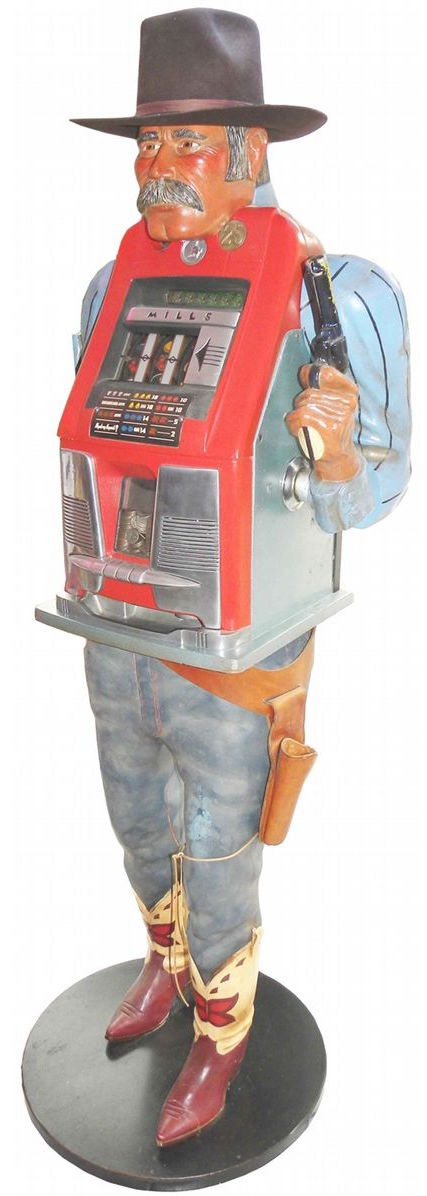
\includegraphics[height=1.01in]{stuff/mab3.jpg}}&
\raisebox{.05\height}{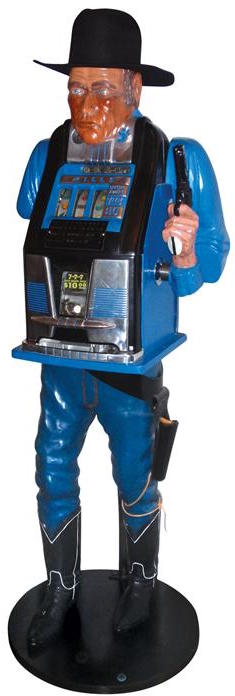
\includegraphics[height=1.1in]{stuff/mab6.jpg}}&
\raisebox{-.02\height}{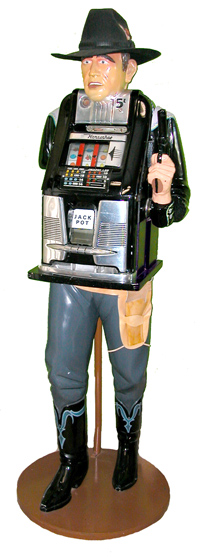
\includegraphics[height=1.25in]{stuff/mab1.jpg}}&
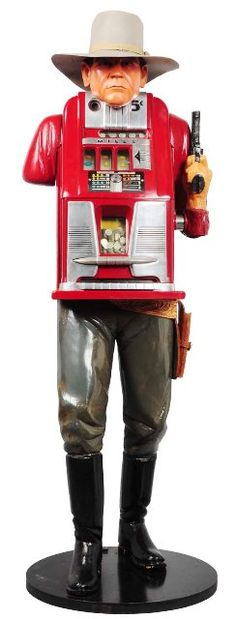
\includegraphics[height=1.3in]{stuff/mab2.jpg}&
\raisebox{0\height}{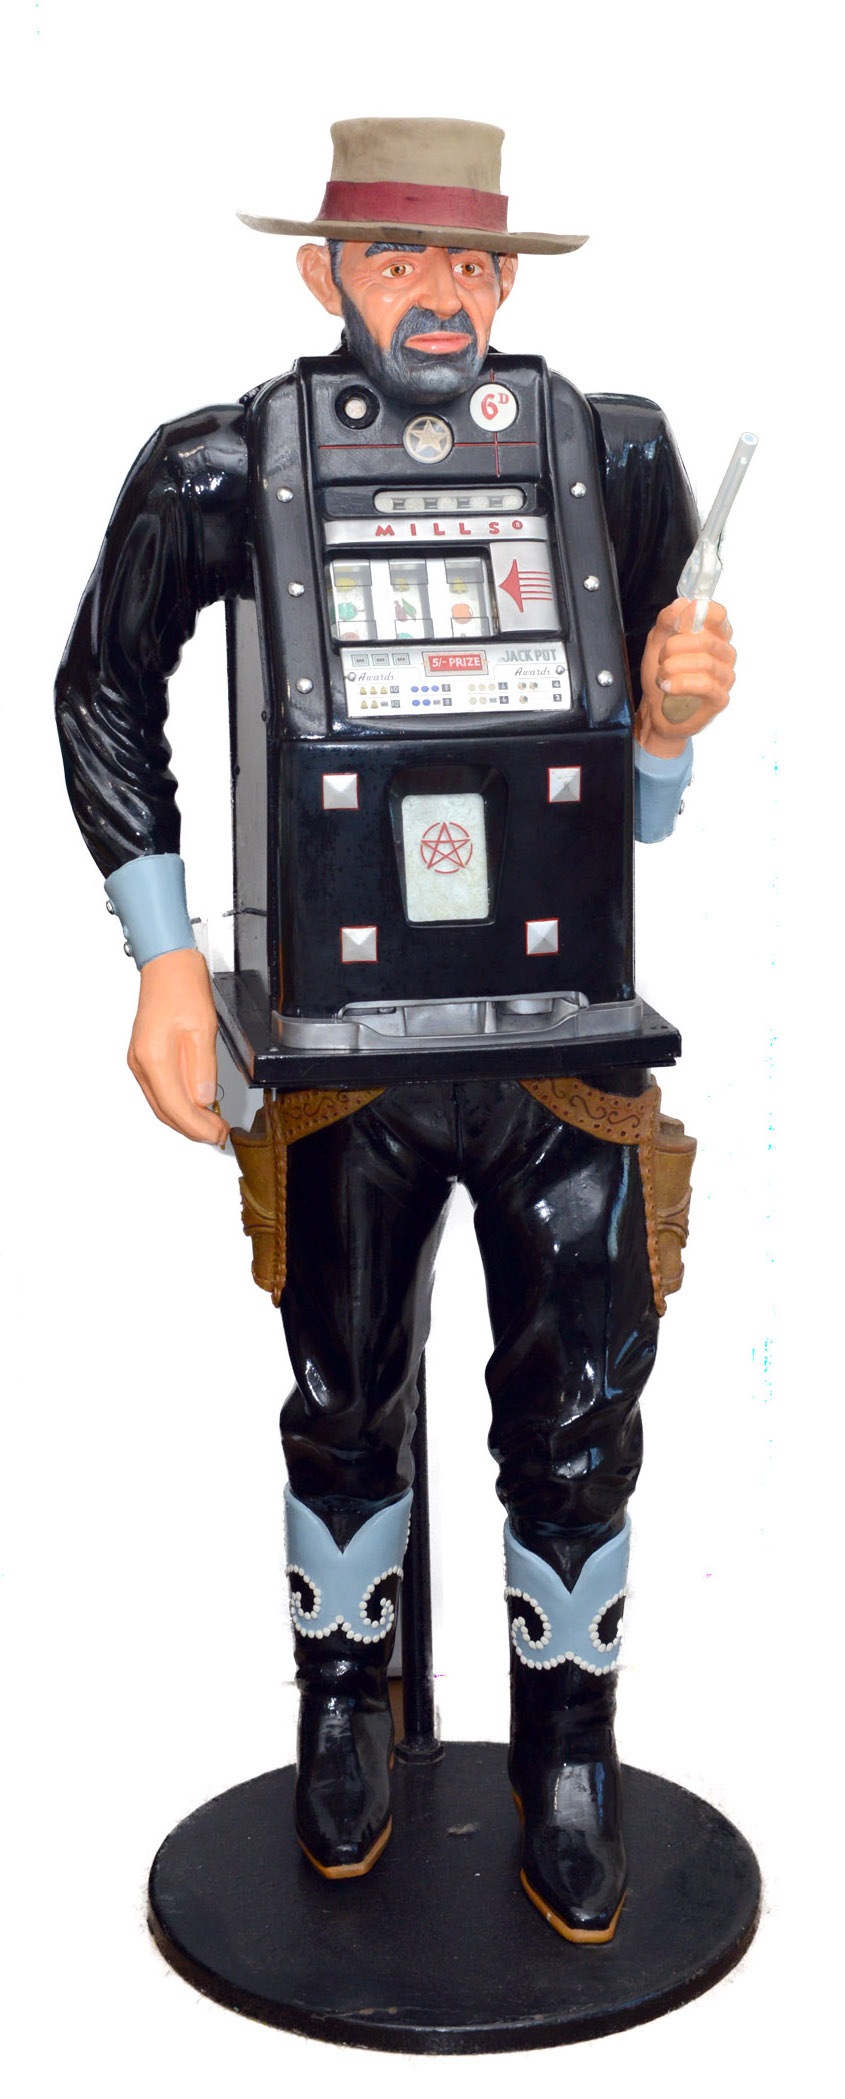
\includegraphics[height=1.25in]{stuff/mab7.jpg}}&
\raisebox{.06\height}{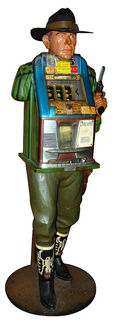
\includegraphics[height=1.1in]{stuff/mab5.jpg}}&     
\raisebox{.1\height}{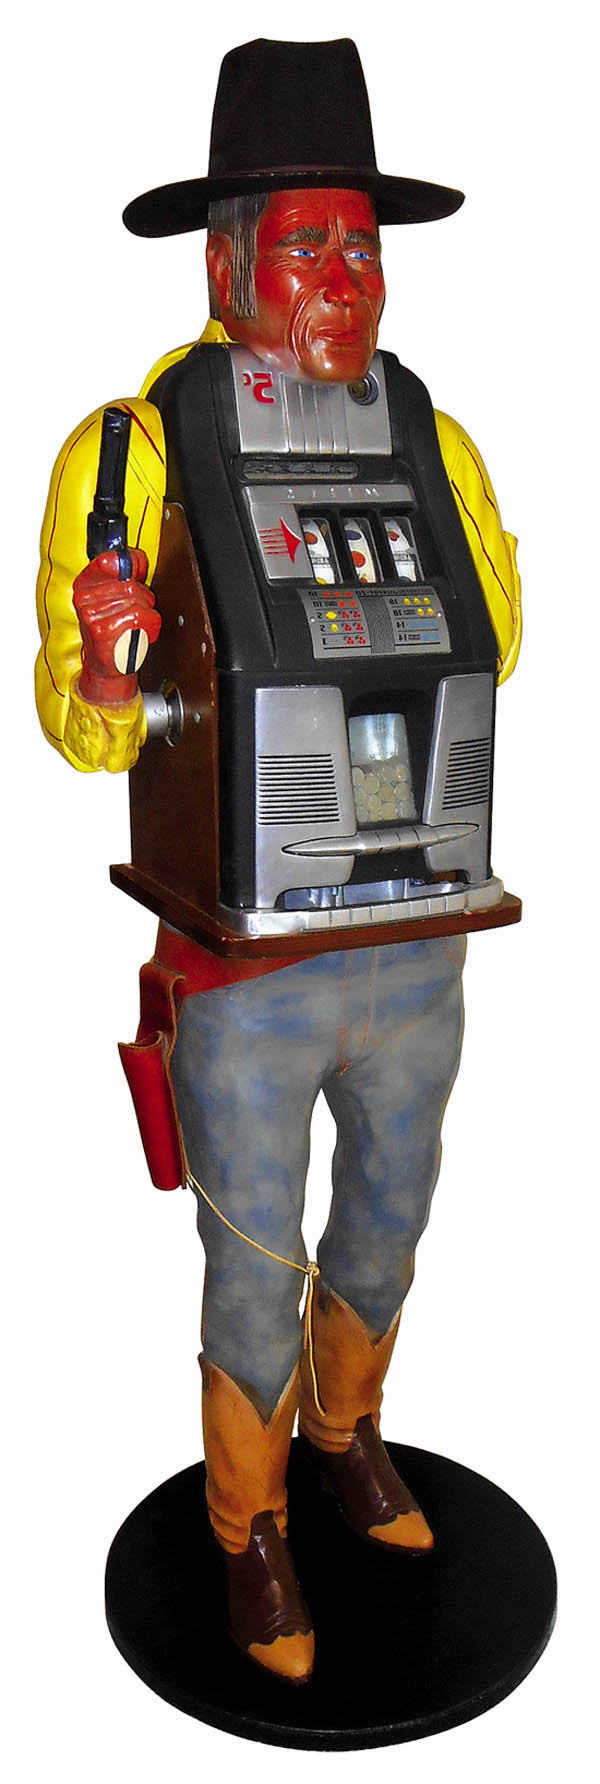
\includegraphics[height=1.03in]{stuff/mab8.jpg}} \\\\\\\\
\end{tabular}}

\vspace{-4em}

\setlength{\leftmargini}{-2pt}
\begin{itemize}
\item[]<3->
\setlength\tabcolsep{-1pt}
\begin{tabular}{llllllll}

\includegraphics[height=.425in]{stuff/p6.png}
&
\includegraphics[height=.425in]{stuff/p5.png}
&
\includegraphics[height=.425in]{stuff/p1.png}
&
\includegraphics[height=.425in]{stuff/p2.png}
&
\includegraphics[height=.425in]{stuff/p4.png}
&
\includegraphics[height=.425in]{stuff/p3.png}
&
\includegraphics[height=.425in]{stuff/p7.png}\\
\end{tabular}
\end{itemize}
}


\frame
{
\frametitle{Objectives}

\Large
\begin{enumerate}%[leftmargin=*]
\item Bayesian versus Frequentist A/B testing \\${}$\\
\item Bayesian Priors\\${}$\\
\item Multi-armed bandit deployment
\begin{itemize}
\item Regret: all about it and having none of it
\item $\epsilon$-greedy, softmax, UCB1, and the Bayesian Bandit
\end{itemize}
\end{enumerate}

}


\frame
{
\frametitle{A/B Testing reminder}
  
\begin{table}
\centering
\begin{tabular}{r|c|c}
&\multirow{4}{*}{
\includegraphics[height=.75in]{stuff/p6.png}}&\multirow{4}{*}{
\includegraphics[height=.75in]{stuff/p2.png}}\\ 
\onslide<7->{$X_{\textcolor{gray}{A}}^{\textcolor{gray}{(i)}} \sim {} \text{Bern}\left(\theta_{\textcolor{gray}{A}}\right)$} & & \\ 
\onslide<7->{$X_{\textcolor{gray}{B}}^{\textcolor{gray}{(j)}} \sim {} \text{Bern}\left(\theta_{\textcolor{gray}{B}}\right)$}  & & \\ 
 & & \\ \hline
Trial 1 & \onslide<2->{$\emptyset$} & \\ 
Trial 2 &  & \onslide<3->{$\emptyset$} \\ 
Trial 3 &  & \onslide<4->{\checkmark} \\ 
Trial 4 & \onslide<5->{$\emptyset$} &  \\ 
$\vdots$ & & \\ 
Trial $n_{\textcolor{gray}{A}} + n_{\textcolor{gray}{B}}$ & &\\  \hline 
Total & \onslide<6->{$\hat p_{\textcolor{gray}{A}} = \frac{\sum X_{\textcolor{gray}{A}}^{\textcolor{gray}{(i)}}}{n_{\textcolor{gray}{A}}}$\hspace{4em}} & \onslide<6->{$\hat p_{\textcolor{gray}{B}} = \frac{\sum X_{\textcolor{gray}{B}}^{\textcolor{gray}{(j)}}}{n_{\textcolor{gray}{B}}}}$\hspace{4em}\\\hline
\end{tabular}
\onslide<7->{$$\hat p_{\textcolor{gray}{A}} - \hat p_{\textcolor{gray}{B}} \sim N\left(\theta_{\textcolor{gray}{A}} - \theta_{\textcolor{gray}{B}}, 
\frac{\theta_{\textcolor{gray}{A}}(1-\theta_{\textcolor{gray}{A}})}{n_{\textcolor{gray}{A}}} + \frac{\theta_{\textcolor{gray}{B}}(1-\theta_{\textcolor{gray}{B}})}{n_{\textcolor{gray}{B}}} \right)$$
$$\text{and if $ \theta_{\textcolor{gray}{A}} = \theta_{\textcolor{gray}{B}} = \theta$ then } \hat p_{\textcolor{gray}{A}} - \hat p_{\textcolor{gray}{B}} \sim N\left(0, \frac{2\hat p(1-\hat p)}{n_{\textcolor{gray}{A}}+n_{\textcolor{gray}{B}}}\right)$$}
\end{table}
}



\frame{
\frametitle{A/B \textbf{Hypothesis Testing} \emph{power calculations} }

\begin{columns}
\begin{column}{.45\textwidth}
\begin{itemize}
\item Effect size is $0.06 - 0.04$
\item With $2n$ alternating trials\\ $\hat p = 0.05$
\item $se = \sqrt{2\frac{\hat p(1 - \hat p)}{n}}$
\item[] 
\end{itemize}
\end{column}
\begin{column}{.55\textwidth}
${}$
\end{column}
\end{columns}


\hspace*{-.75cm}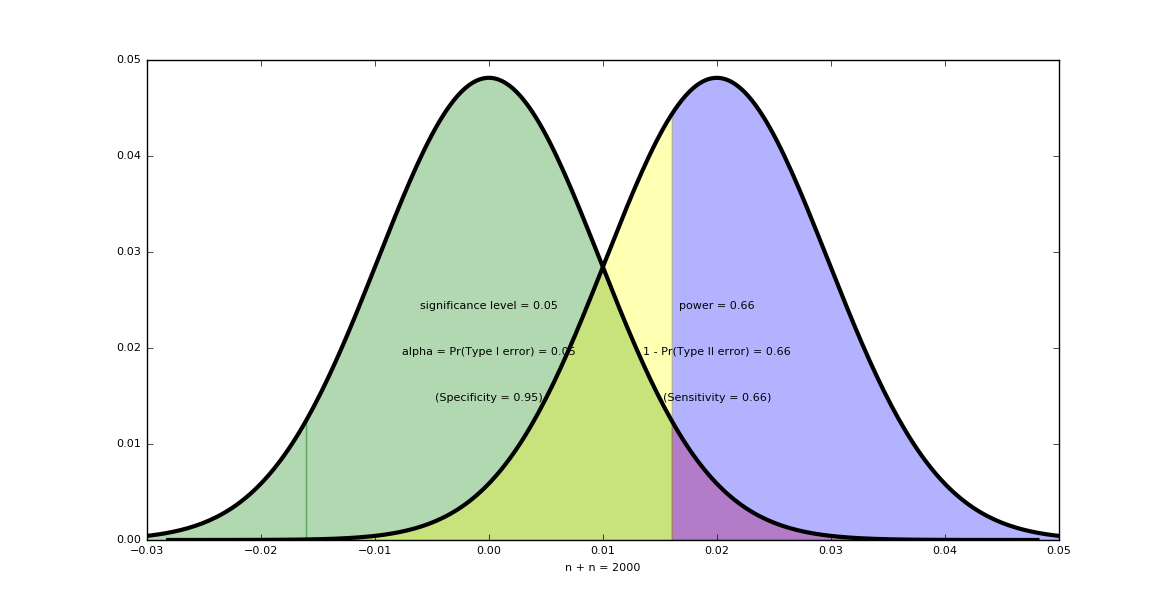
\includegraphics[height=1.55in]{stuff/power_2.png}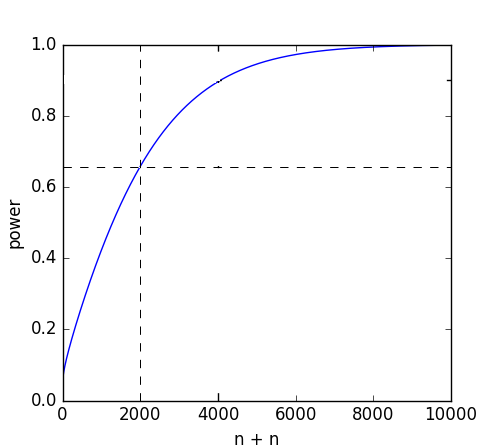
\includegraphics[height=1.55in]{stuff/figure_2.png}
%\raisebox{.0\height}{}
}


\frame{
\frametitle{A/B \textbf{Hypothesis Testing} \emph{power calculations} }

\begin{columns}
\begin{column}{.45\textwidth}
\begin{itemize}
\item Effect size is $0.06 - 0.04$
\item With $2n$ alternating trials\\ $\hat p = 0.05$
\item $se = \sqrt{2\frac{\hat p(1 - \hat p)}{n}}$
\item[] 
\end{itemize}
\end{column}
\begin{column}{.55\textwidth}
\onslide<2->{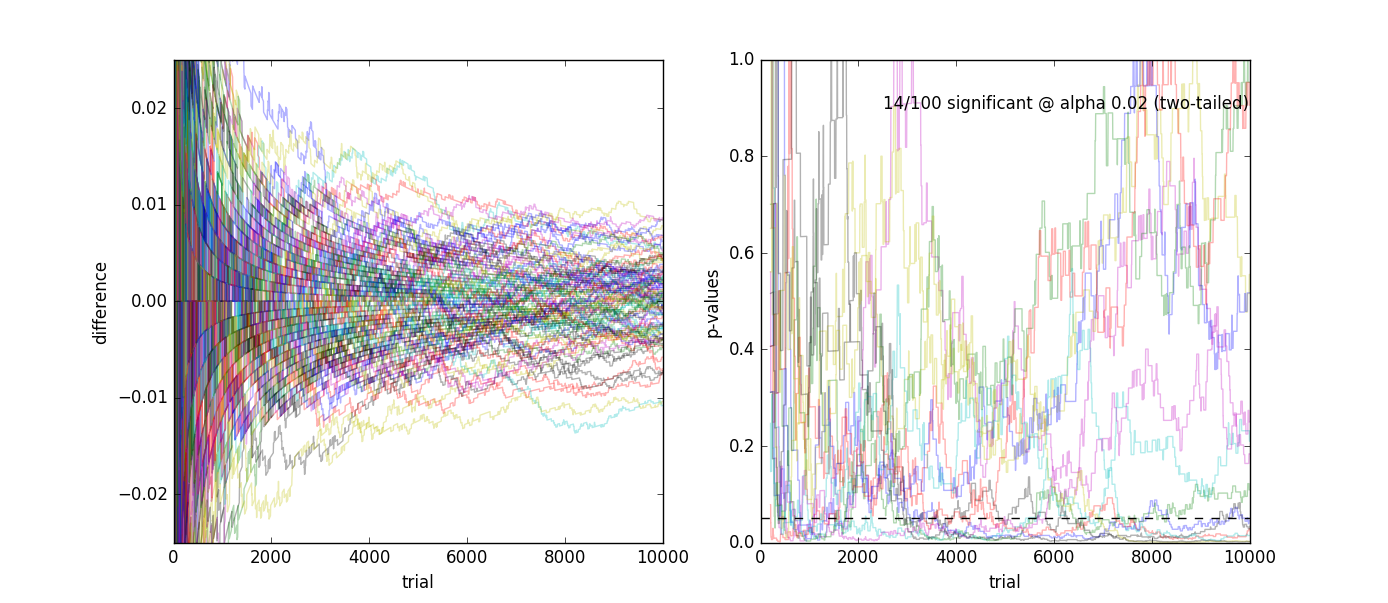
\includegraphics[height=1.1in]{stuff/figure_1.png}}
\end{column}
\end{columns}

\hspace*{-.75cm}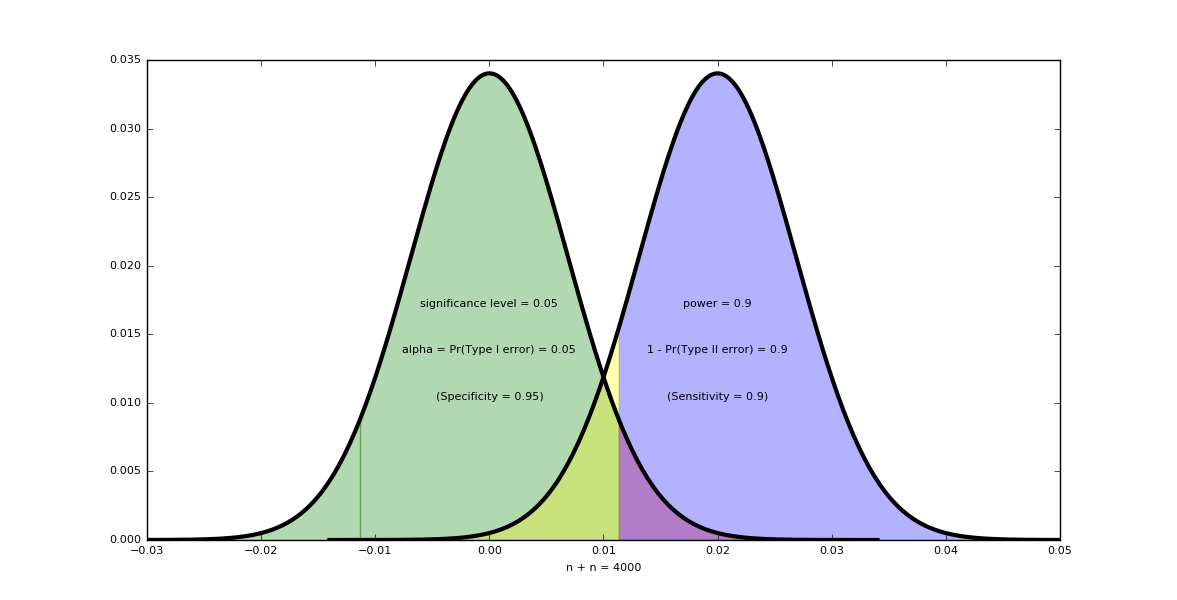
\includegraphics[height=1.55in]{stuff/power_1.png}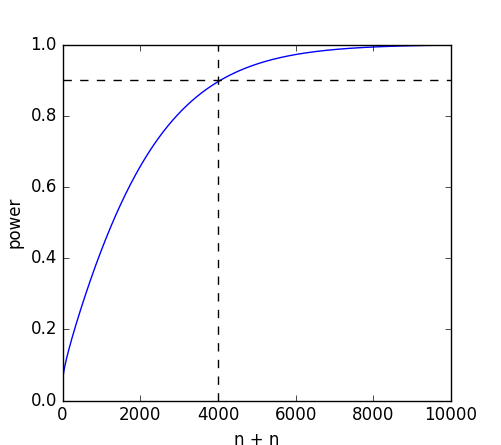
\includegraphics[height=1.55in]{stuff/figure_2b.png}
%\raisebox{.0\height}{}
}




\frame
{
\frametitle{Bayesian \emph{Philosophy}}

  \begin{itemize}
  \item<1-> Rather than $\theta_A$ \& $\theta_B$ being \underline{fixed} constants to be estimated...
  \item<2-> they are \underline{random variables} with distributions $p(\theta_A)$ \& $p(\theta_B)$ \\
%  \textcolor{gray}{E.g., each time a customer arrives at landing page [$A, B$] \\
%  the probability of conversion is drawn from [$f(\theta_A), f(\theta_B)$]}
  \item[]<2-> 
%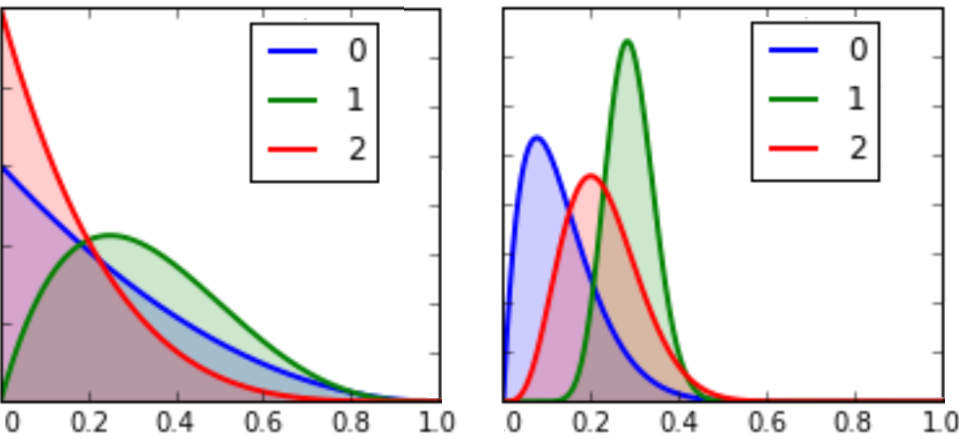
\includegraphics[height=1.7in]{distcomp.png}

\begin{figure}
\centering
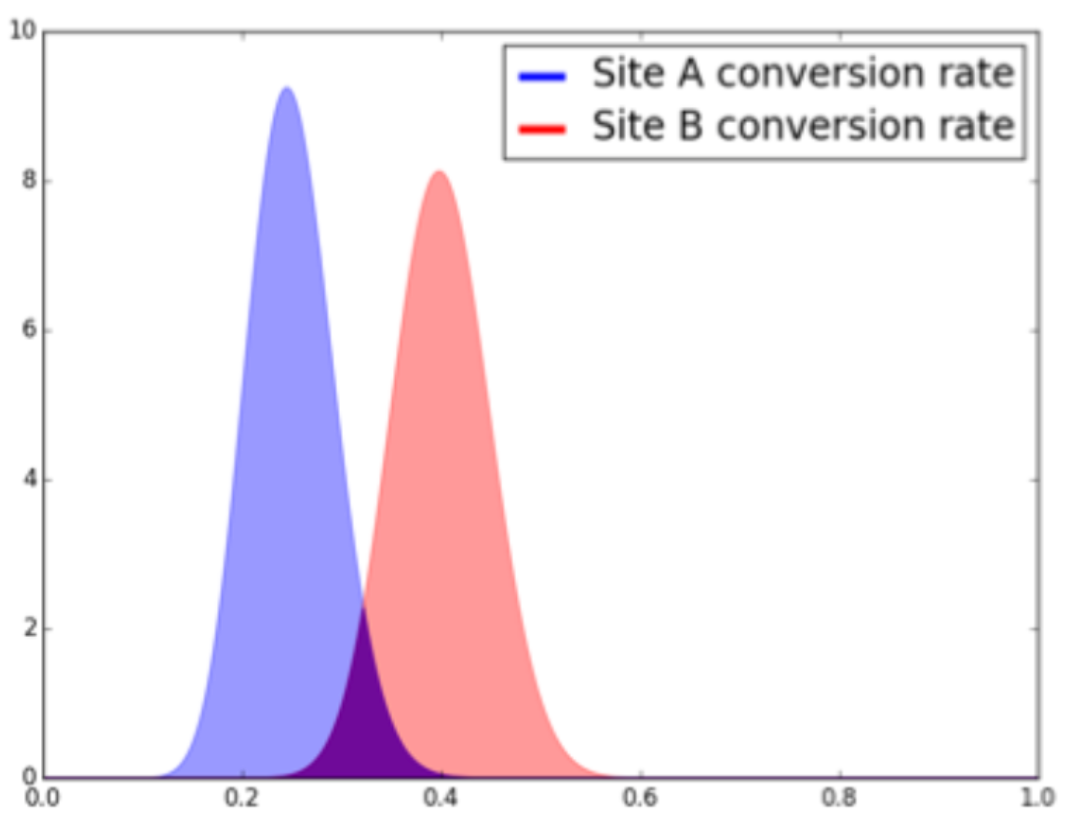
\includegraphics[height=1.5in]{stuff/priors.png}
\end{figure}

  \item<3->  The distributions model the parameter uncertainty given data
  \item<3->  And give probability statements of beliefs about parameters 
  \item<4->[]  \textcolor{red}{E.g., $Pr(\theta_A > \theta_B), Pr(\theta_A - \theta_B > 0.05)$, or $Pr(\frac{\theta_A}{\theta_B}>1.1)$}\\${}$
  \item<5-> Previously, confidence intervals/p-values characterized the (sampling) variability of statistical estimation procedures
  
 %   Interest is in which distribution produces more conversions \\
   
\end{itemize}
}

\frame
{
\frametitle{Questions snarky Bayesians ask Frequentists}


\begin{itemize}
\item Can you say ``there's 95\% probability that A beats B''? \\\onslide<2->{\textcolor{gray}{Nope. But I can.}}\\${}$
\item<3-> Can you stop the test early based on surprising results? \\\onslide<4->{\textcolor{gray}{Nope. But I can.}}\\${}$
\item<5-> Can you update the test parameters while it's running? \\\onslide<6->{\textcolor{gray}{Nope. But I can.}}
\end{itemize}


}




\frame
{
\frametitle{Bayesian \emph{Theory}}

\begin{itemize}
\item Data $X$ that informs our knowledge of $\theta_A$ and $\theta_B$ 
allows us to ``update'' our beliefs about $\theta_A$ and $\theta_B$ using \emph{Bayes' Theorem}
$$\textcolor{ForestGreen}{f(\theta|X)} = \frac{\textcolor{orange}{f(X|\theta)}\textcolor{RoyalBlue}{f(\theta)}}{\textcolor{gray}{f(X)}}$$
\item<2-> Bayes' Theorem derives the \textcolor{ForestGreen}{posterior (theta given data)} as a function of the
\textcolor{orange}{likelihood}, the \textcolor{RoyalBlue}{prior} and the \textcolor{gray}{marginal likelihood}
\item<3-> The posterior is \textcolor{gray}{(marginal likelihood)} proportional to:
$$\textcolor{ForestGreen}{f(\theta|X)} \propto \textcolor{orange}{f(X|\theta)}\textcolor{RoyalBlue}{f(\theta)}$$
\end{itemize}

\vspace{-2.5em}
\begin{figure}
\centering
\onslide<4->{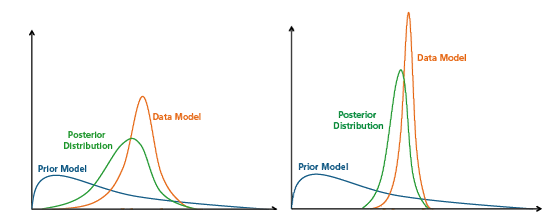
\includegraphics[height=1.5in]{stuff/bayes.png}}
\end{figure}

}


\frame
{
\frametitle{Beta Distribution}

\begin{figure}
\centering
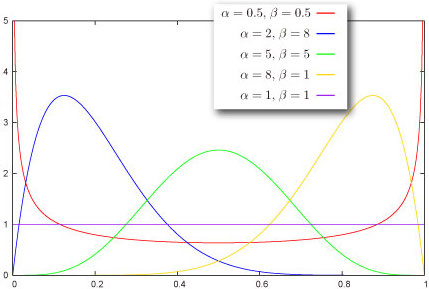
\includegraphics[height=2.25in]{stuff/plotBeta.jpg}
\end{figure}
\Huge$$\frac{\Gamma(\alpha+\beta)}{\Gamma(\alpha)+\Gamma(\beta)}\theta^{\alpha - 1}(1-\theta)^{\beta - 1}$$

}

\frame
{
\frametitle{Bayesian A/B Testing}

\begin{itemize}
\item \textcolor{orange}{Likelihood}
\begin{align*}   
f(X_1,X_2,\cdots,X_n|\theta) = {}& f(X_1|\theta)f(X_2|\theta) \cdots f(X_n|\theta) \\
= {}& \prod_{i=1}^n \theta^{X_i}(1-\theta)^{1-X_i} \quad\quad\quad\;\; \textcolor{pink}{\text{[beta(s)]}} \\
= {}& \textcolor{orange}{\theta^{\overset{\tiny n}{\underset{\tiny i=1}{\sum}} X_i}(1-\theta)^{n-\overset{\tiny n}{\underset{\tiny i=1}{\sum}} X_i}}
\end{align*}   

\item<2->  \textcolor{pink}{Conjugate}* \textcolor{RoyalBlue}{Prior}
\begin{align*}   
f(\theta) = {}& \textcolor{gray}{\frac{\Gamma(\alpha+\beta)}{\Gamma(\alpha)+\Gamma(\beta)}}\textcolor{RoyalBlue}{\theta^{\alpha - 1}(1-\theta)^{\beta - 1}} \quad\quad\quad\quad\quad\; \textcolor{pink}{\text{[beta]}}
\end{align*}   

\item <3-> \textcolor{ForestGreen}{Posterior}

\begin{align*}   
\textcolor{ForestGreen}{f(\theta|X)} \propto {}& \textcolor{orange}{\theta^{\sum X_i}(1-\theta)^{n-\sum X_i}}\textcolor{RoyalBlue}{\theta^{\alpha - 1}(1-\theta)^{\beta - 1}} \\
= {}& \textcolor{ForestGreen}{\theta^{\alpha + \sum X_i - 1}(1-\theta)^{\beta + n-\sum X_i - 1}} \quad\quad\quad\quad \textcolor{pink}{\text{[beta]}}
\end{align*}   


\end{itemize}
}


\frame
{
\frametitle{Beta Distribution Updates}
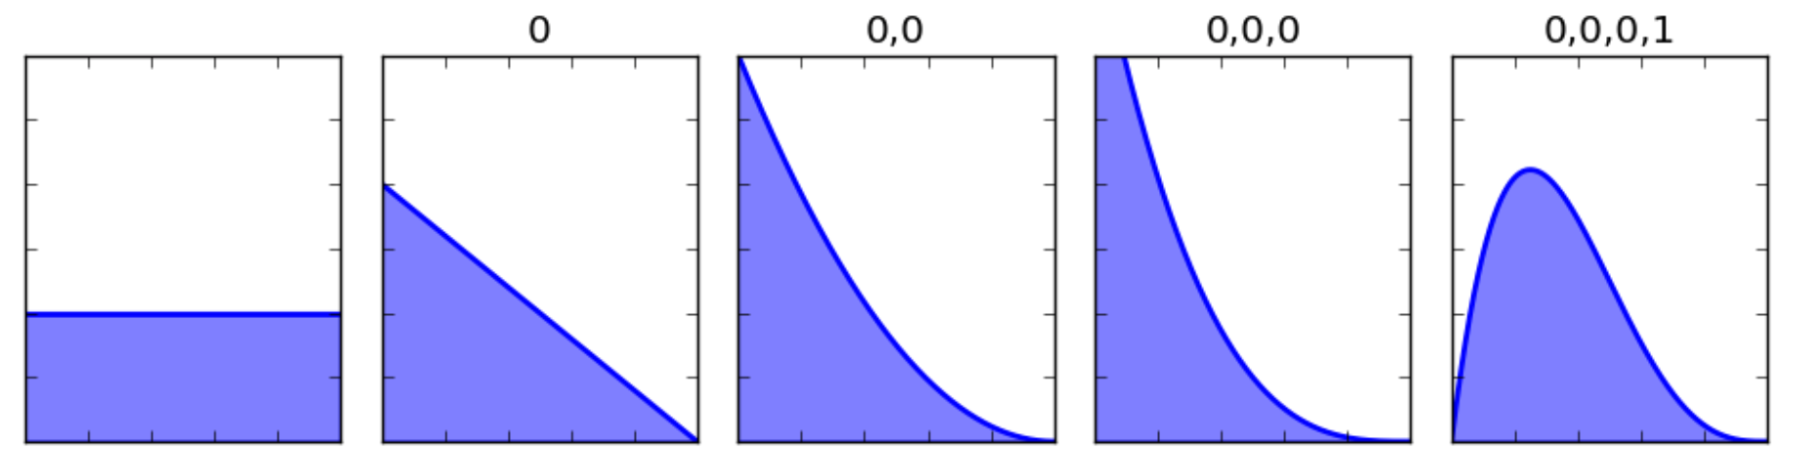
\includegraphics[width=4.2in]{stuff/beta_updates.png}

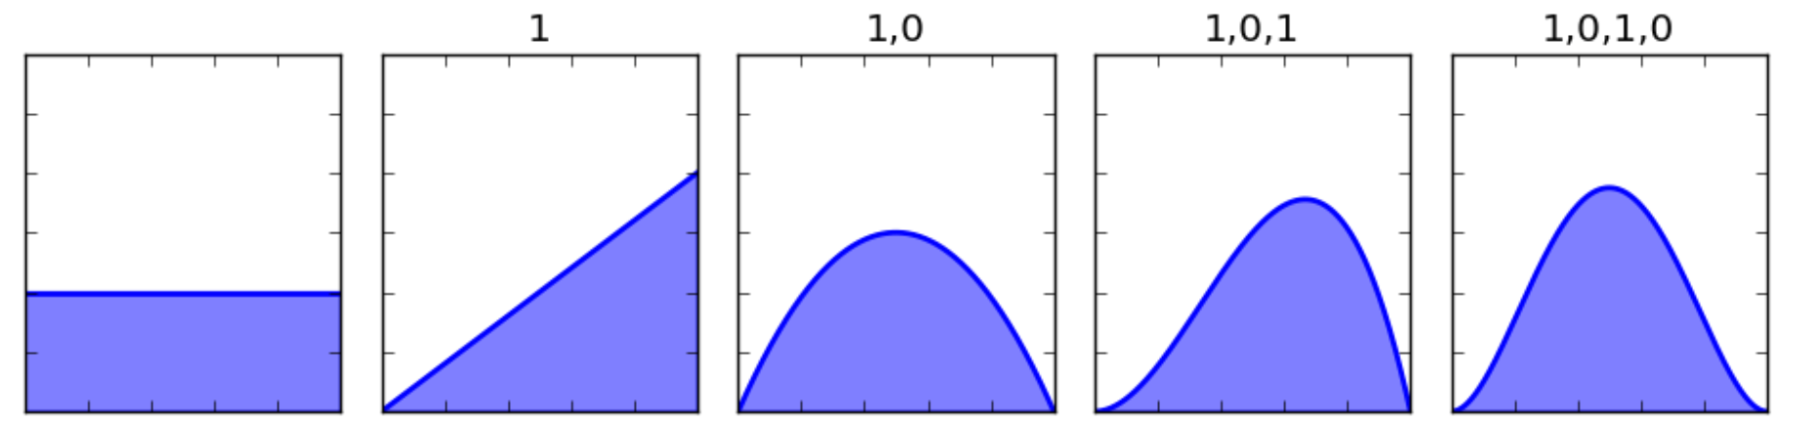
\includegraphics[width=4.2in]{stuff/beta_updates1.png}

\huge
$$\text{Beta}\left(\alpha + \sum X_i, \beta + n-\sum X_i\right)$$
}


\frame
{
\frametitle{Beta Distribution Updates}


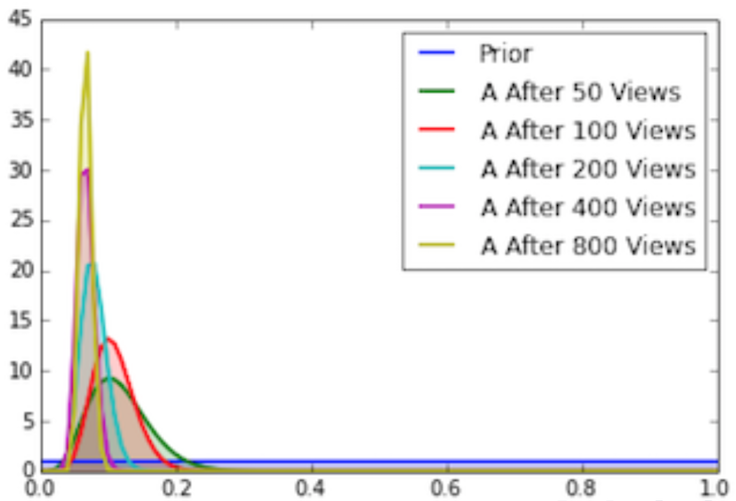
\includegraphics[height=1.75in]{stuff/bayesian-updates-1.png}\hspace{0.4em}\raisebox{.5em}{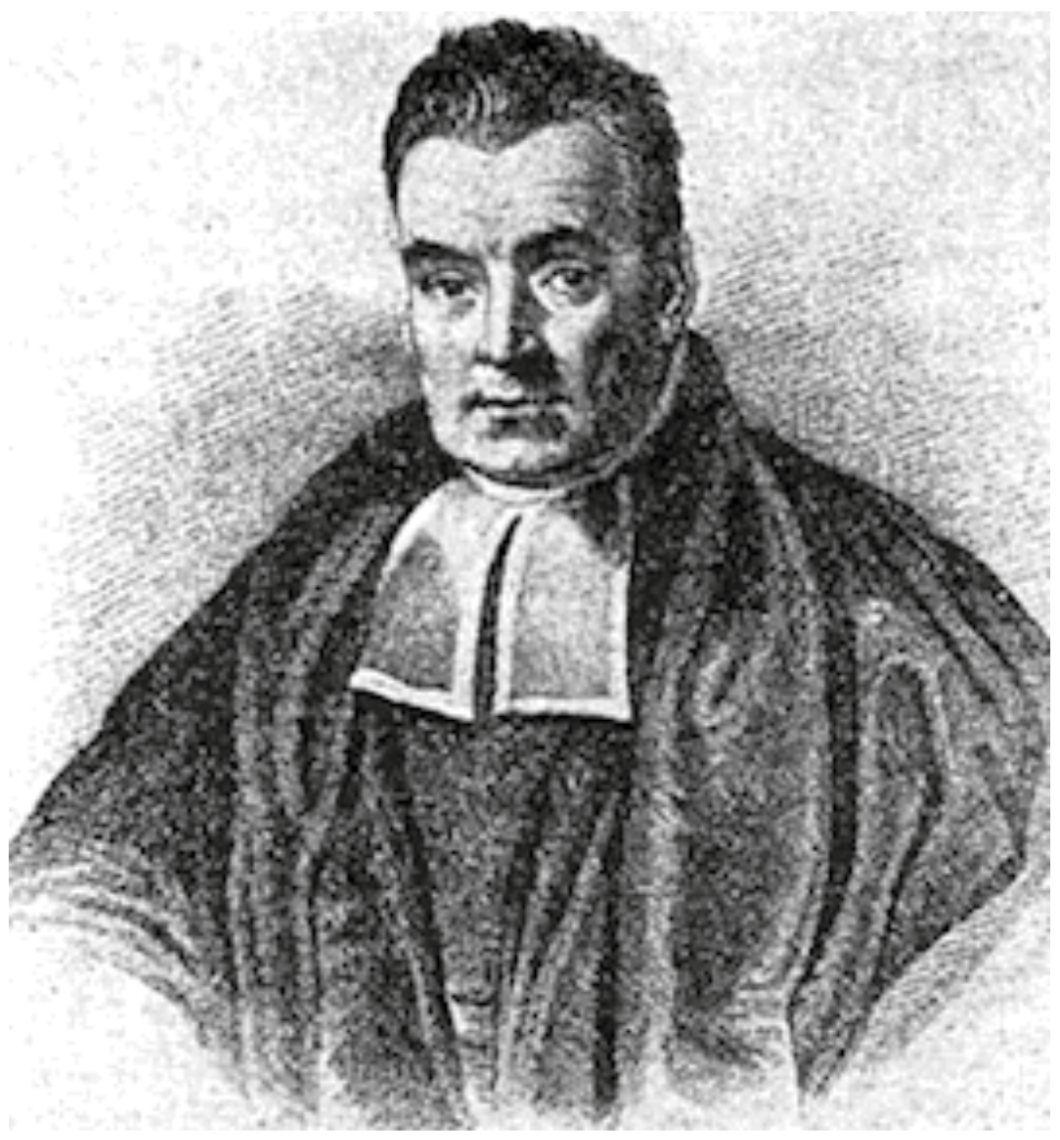
\includegraphics[height=1.66in]{stuff/bayes2.png}}


\hspace{6em}\tiny Probability of Success\hspace{11em} Rev. Thomas Bayes (1701 -- 1761) \\ ${}$\\

\large
$$\textcolor{ForestGreen}{f(\theta|X)} = \frac{\textcolor{orange}{f(X|\theta)}\textcolor{RoyalBlue}{f(\theta)}}{\textcolor{Gray}{f(X)}} = \text{Beta}\left(\alpha + \sum X_i, \beta + n-\sum X_i\right)$$


}






\frame
{
\frametitle{A brief synopsis of the world of the world to date}

\vspace{-.9in}
\begin{figure}
\centering
\onslide<2->{\raisebox{.6em}{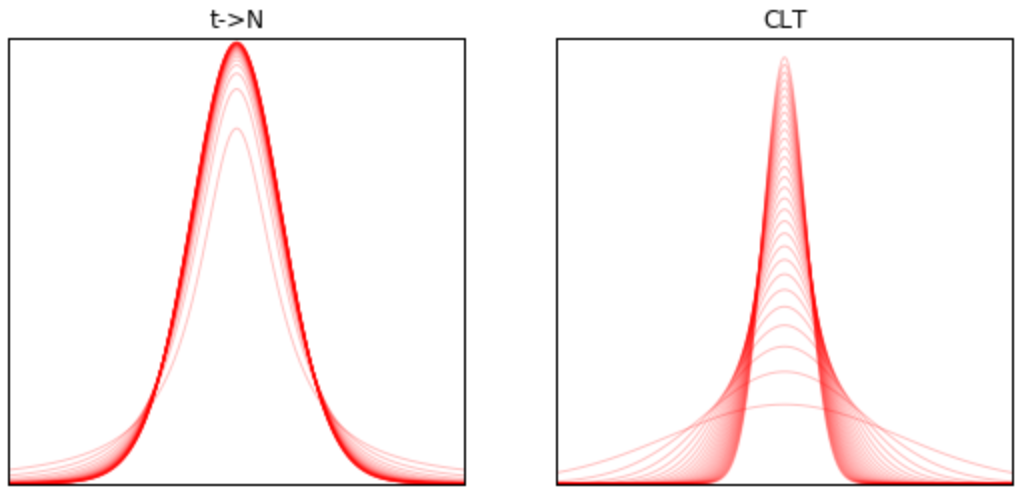
\includegraphics[height=.95in]{stuff/assymp.png}}}$\quad\quad$\onslide<3->{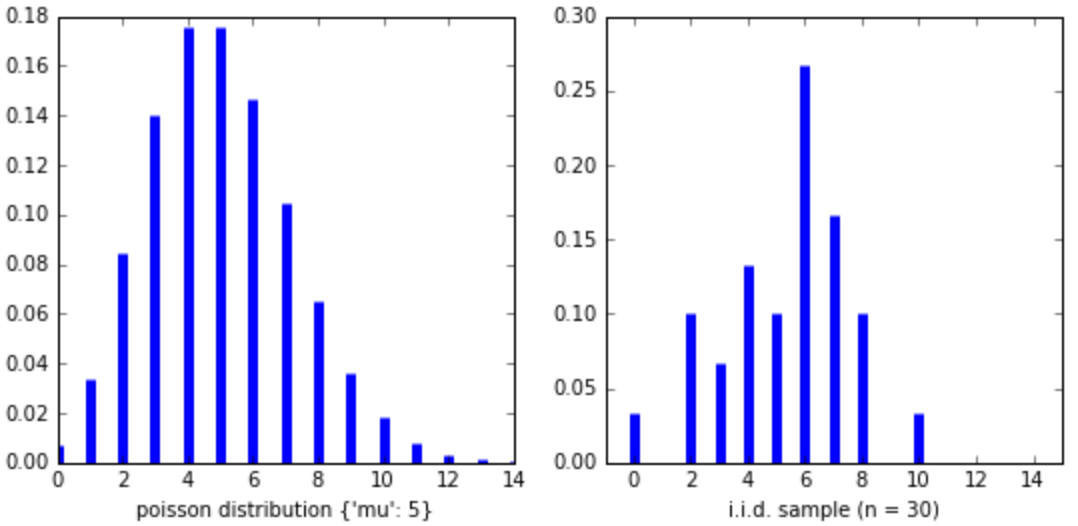
\includegraphics[height=1in]{stuff/boots.png}}\\
\onslide<2->{\quad\quad$n \longrightarrow \infty \;\quad\quad\quad\quad\quad\quad\quad\quad\quad\quad}\onslide<3->{\text{nonparametrics}$}
\end{figure}
\vspace{-.25in}
\hspace*{-.15in}\onslide<4->{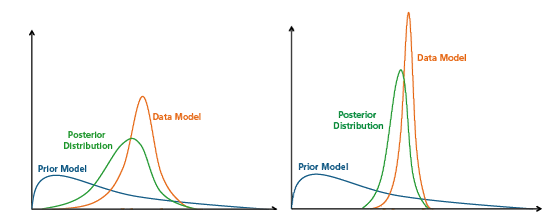
\includegraphics[height=1.75in]{stuff/bayes.png}}


\vspace{-1.45in}
\onslide<4->{
{$\arraycolsep=1.4pt
\quad\;\begin{array}{rcl}
\textcolor{ForestGreen}{Posterior} &\propto & \textcolor{orange}{Likelihood} \times \textcolor{RoyalBlue}{Prior}\\
\textcolor{ForestGreen}{f(\theta | X)} &\propto & \textcolor{orange}{f(X | \theta)} \times \textcolor{RoyalBlue}{f(\theta)} 
\end{array}$}
}
}


\frame
{
\frametitle{Parametric Versus Nonparametric}

We might characterize an analysis framework as parametric if

\begin{enumerate}
\setlength\itemsep{.75em}
\item Results are buttressed or bolstered by modeling assumptions 
\onslide<2->{\textcolor{gray}{\emph{E.g. leveraging the structure of normality via a z-test increases power but comes at a cost of 
loss of robustness compared to 
nonparametric tests free of distributional assumptions.} 
}}
\item<3-> Predicted values are based on ``parameters.'' \\
\onslide<4->{\textcolor{gray}{\emph{E.g., the $\beta$ coefficients in linear regression.}}}
\item<5-> Parameter estimation  
determines the specific instance of a model within a ``model class'' defined by those parameters. \\
\onslide<6->{\textcolor{gray}{\emph{E.g., the CLT guarantees a normal distribution which is determined by estimating $\mu$ and $\sigma^2/\sqrt{n}$ with $n$  large}}}
\item<7-> The complexity of the model does grows as data size $n$ grows.
\onslide<8->{\textcolor{gray}{\emph{E.g. trees grow in complexity as data becomes richer while a normal distribution is defined by $\mu$ and $\sigma^2$ regardless of $n$.}}}
\end{enumerate}
}



\frame
{
  \frametitle{The Multi-Armed Bandit}

\begin{tabular}{ccccccc}
\raisebox{.1\height}{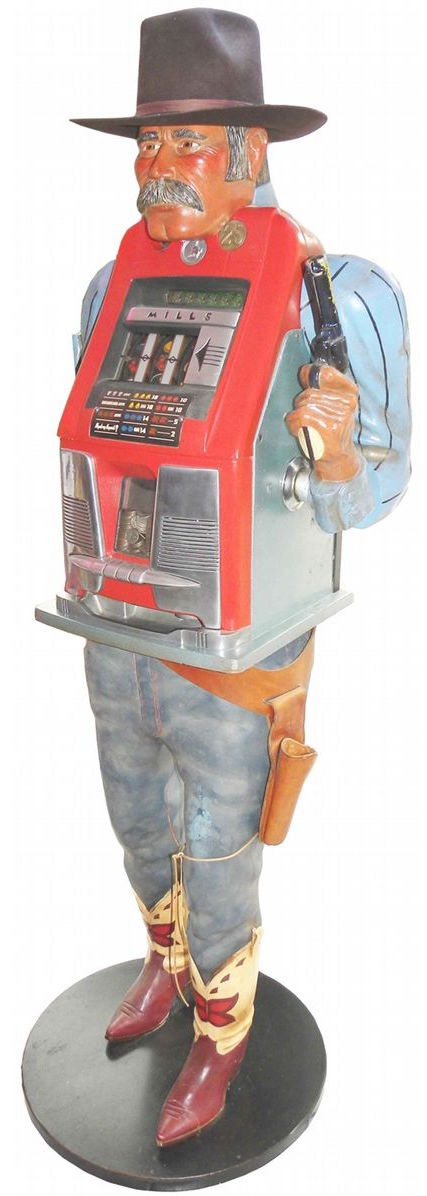
\includegraphics[height=1.01in]{stuff/mab3.jpg}}&
\raisebox{.05\height}{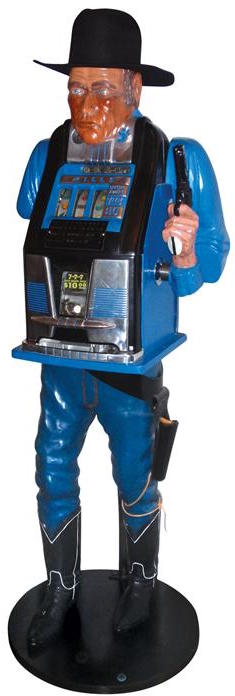
\includegraphics[height=1.1in]{stuff/mab6.jpg}}&
\raisebox{-.02\height}{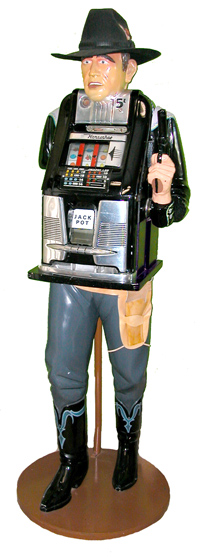
\includegraphics[height=1.25in]{stuff/mab1.jpg}}&
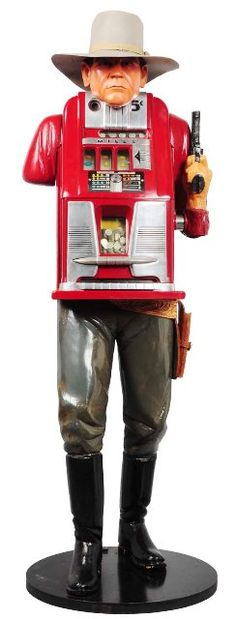
\includegraphics[height=1.3in]{stuff/mab2.jpg}&
\raisebox{0\height}{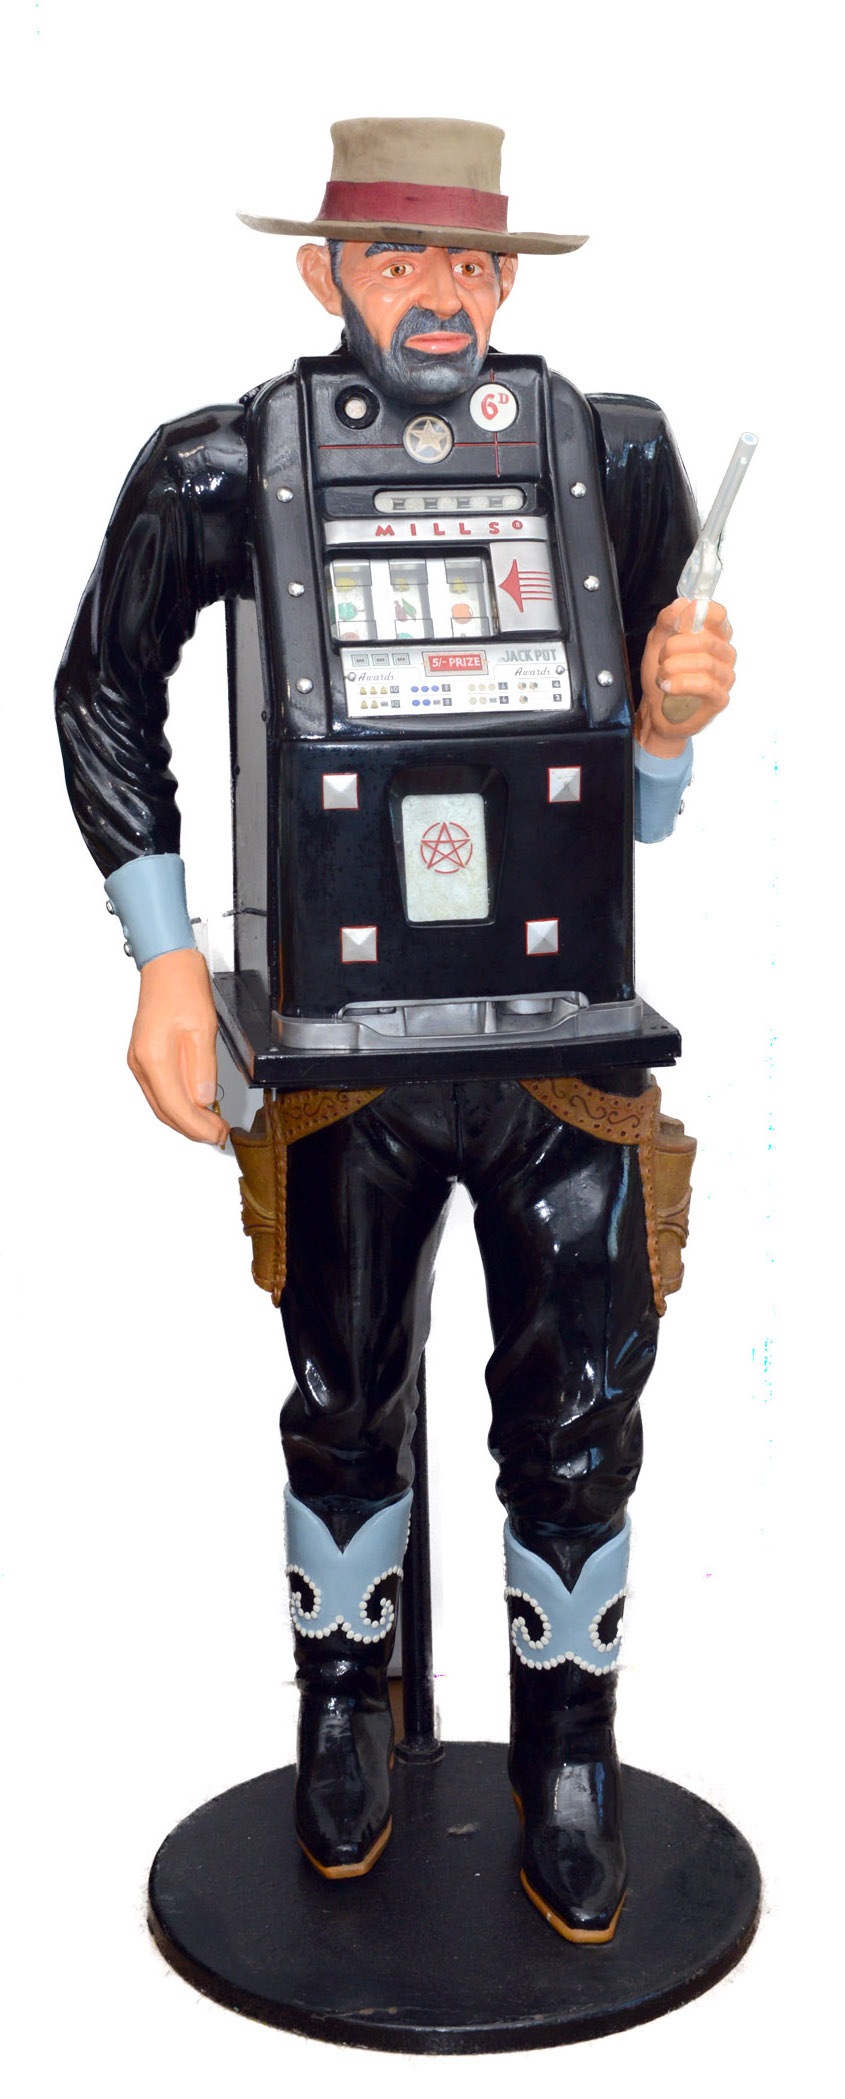
\includegraphics[height=1.25in]{stuff/mab7.jpg}}&
\raisebox{.06\height}{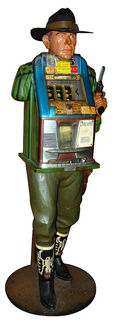
\includegraphics[height=1.1in]{stuff/mab5.jpg}}&     
\raisebox{.1\height}{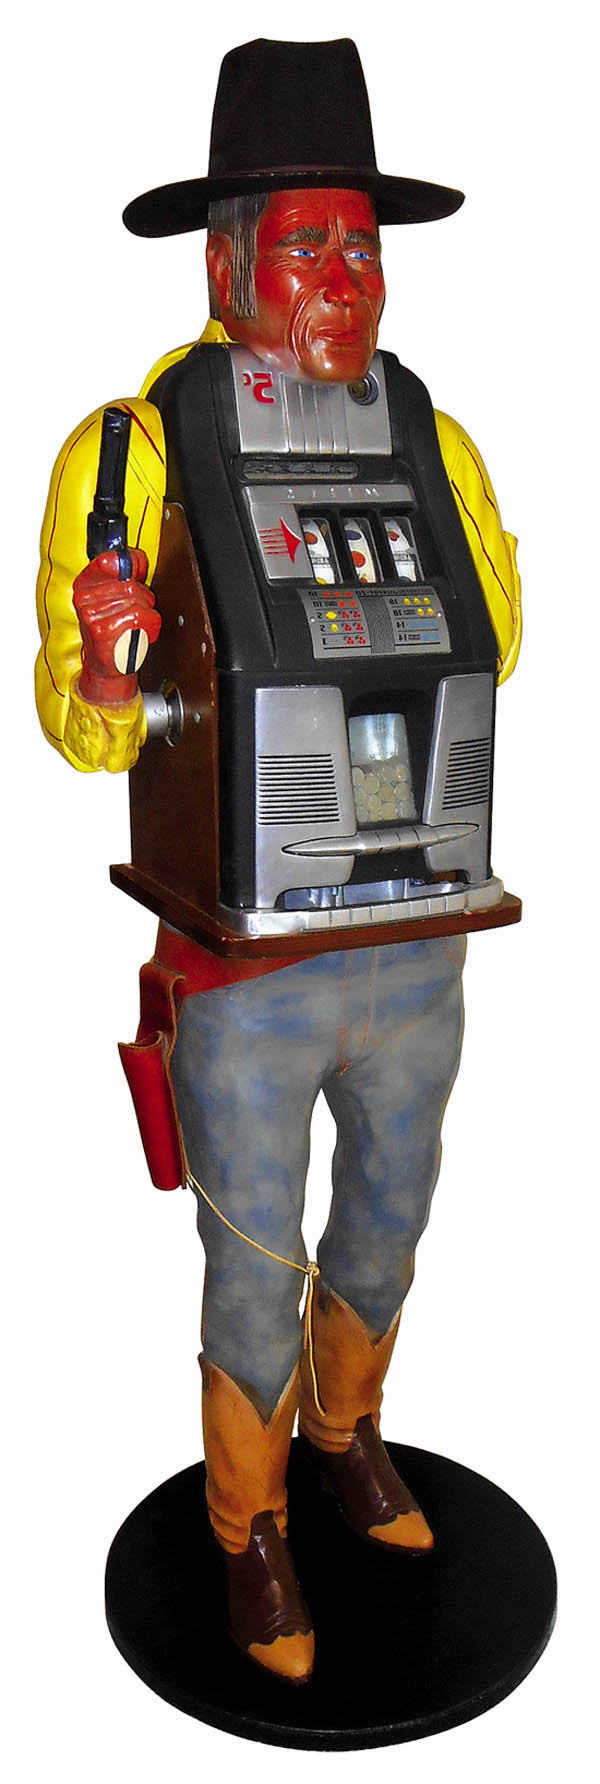
\includegraphics[height=1.03in]{stuff/mab8.jpg}} \\\\
\end{tabular}


\setlength{\leftmargini}{-15pt}
\begin{itemize}
\item[]<2->
\setlength\tabcolsep{-1pt}
\begin{tabular}{r|lllllll}
&
\includegraphics[height=.425in]{stuff/p6.png}
&
\includegraphics[height=.425in]{stuff/p5.png}
&
\includegraphics[height=.425in]{stuff/p1.png}
&
\includegraphics[height=.425in]{stuff/p2.png}
&
\includegraphics[height=.425in]{stuff/p4.png}
&
\includegraphics[height=.425in]{stuff/p3.png}
&
\includegraphics[height=.425in]{stuff/p7.png}\\
$\frac{\text{Truth}}{\text{Trial}}$ & $\;\;$0.01 & $\;\;$0.02 & $\;\;$0.04 & $\;\;$0.03 & $\;\;$0.05 & $\;\;$0.04 & $\;\;$0.02\\ \hline
 1$\;\;$ &  & \\ 
2$\;\;$ &  &  \\ 
$\vdots\;\;$ & \\ 
\end{tabular}

\item[]<3->
\vspace{-.5in}
\Huge
$\quad\;\;$ \textcolor{red}{Exploration \& Exploitation}
\end{itemize}

}



\frame
{
\frametitle{The Multi-Armed Bandit and \textcolor{Maroon}{\emph{Regret}}}

\Huge
\begin{align*}
\text{regret} = {}& \overset{T} {\underset{t}{\sum}} \underset{k}{\text{max }} \theta_k - \theta^{(t)} \\
 = {}& \textcolor{gray}{T \cdot \underset{k}{\text{max }} \theta_k - \overset{T}{\underset{t}{\sum}} \theta^{(t)}}
\end{align*}
}




\frame
{
\frametitle{The Multi-Armed \textcolor{Maroon}{\emph{random}} Bandit}


Random: \emph{A/B\textcolor{gray}{[/C/D/E/F/G]}-test}\\\textcolor{gray}{[when should you test?]}


\begin{figure}
\centering
\noindent 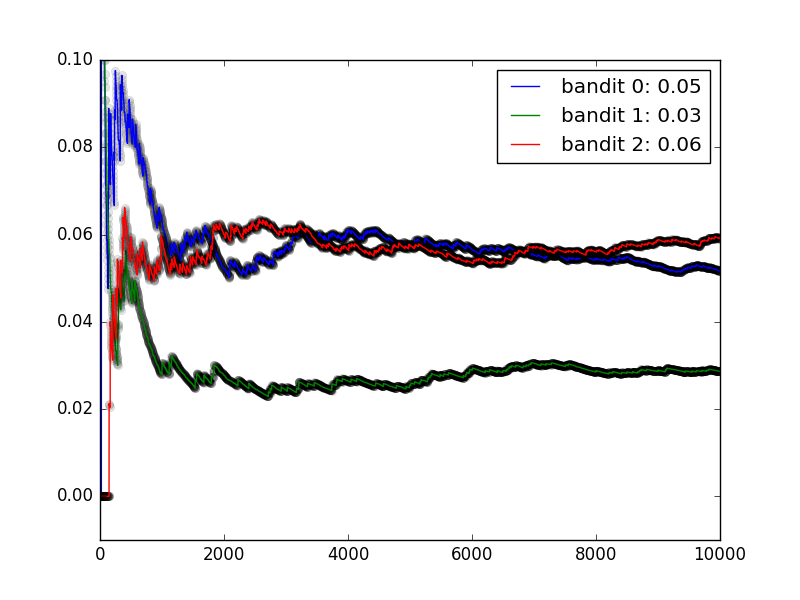
\includegraphics[height=3in]{stuff/mab_ran.png}
\end{figure}
}





\frame
{
\frametitle{The Multi-Armed  \textcolor{Maroon}{\emph{max}} Bandit}


Max: \emph{use the (currently) best performing option}\\\textcolor{gray}{[perhaps after a burn-in?]} 


\begin{figure}
\centering
\noindent 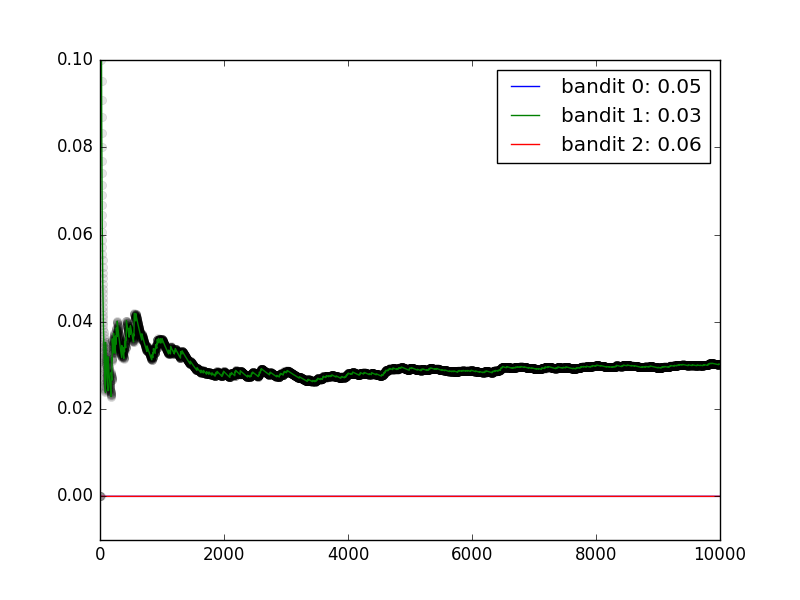
\includegraphics[height=3in]{stuff/mab_max.png}
\end{figure}
}



\frame
{
\frametitle{The Multi-Armed \textcolor{Maroon}{\emph{softmax}} Bandit}

\vspace{.5em}
\begin{columns}
   \begin{column}{0.5\textwidth}
\setlength{\leftmargini}{9pt}
\vspace{-25pt}
\begin{itemize}
\item[] 
\item[] Softmax: \emph{Select proportionally to the currently estimated success rates} 
\vspace{3.85em}
\end{itemize}

\end{column}
\begin{column}{0.5\textwidth}

\vspace{-2.8em}
$\text{Pr}(\text{select } k) \propto  \exp(\hat p_k/\tau), \text{ i.e.,}$\\
${}$\\
$\text{Pr}(\text{select } k) =  \frac{\exp(\hat p_k/\tau)}{\sum \exp(\hat p_k/\tau)}$
        \end{column}
\vspace{-1.5em}
\end{columns}

\vspace{-.42in}
\hspace*{.5em} 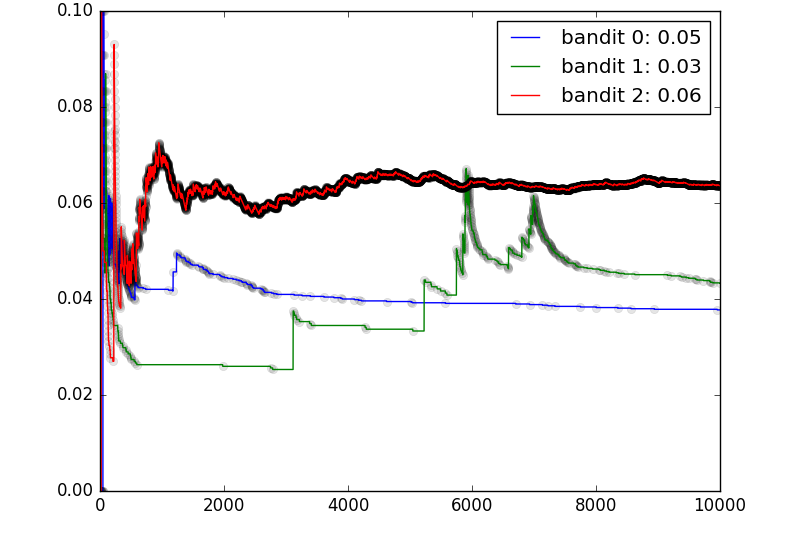
\includegraphics[height=2.755in]{stuff/mab_sm.png}


}



\frame
{
\frametitle{The Multi-Armed  \textcolor{Maroon}{\emph{$\epsilon$-greedy}} Bandit}

$\epsilon$-greedy: \emph{Select randomly with probability $\epsilon$ \\$\quad\quad\quad\quad$otherwise use the current best  option} 

\begin{figure}
\centering
\noindent 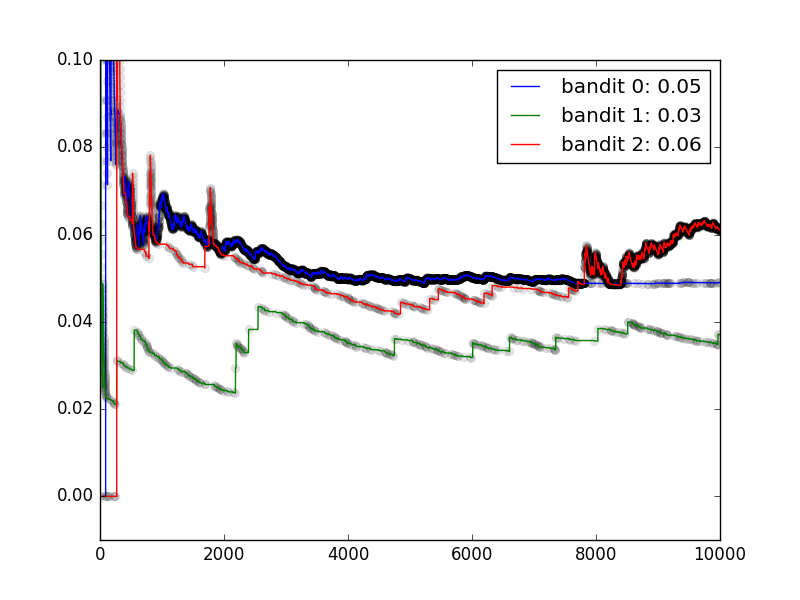
\includegraphics[height=3in]{stuff/mab_epg.png}
\end{figure}

}







\frame
{
\frametitle{The Multi-Armed \textcolor{Maroon}{\emph{UCB1}} Bandit}


\vspace{.5em}
\begin{columns}
   \begin{column}{0.5\textwidth}
\setlength{\leftmargini}{9pt}
\vspace{-25pt}
\begin{itemize}
\item[] 
\item[] UCB1: \emph{Select the option which has the highest \textbf{possible} conversion potential} 
\vspace{3.85em}
\end{itemize}

\end{column}
\begin{column}{0.5\textwidth}

\vspace{-3.4em}
$\underset{k}{\text{max}} \hat p_k + \sqrt{\frac{2 log \sum n_k}{n_k}}$\\
\text{}\\
\text{with $n_k$ trials for bandit $k$}\\
\vspace{1em}
    
    \end{column}
\end{columns}


\vspace{-.46in}
\hspace*{.5em} \includegraphics[height=2.765in]{stuff/mba_ucb1.png}


}



\frame
{
\frametitle{The Multi-Armed \textcolor{Maroon}{\emph{Bayesian}} Bandit}

\setlength{\leftmargini}{0pt}
\begin{itemize}
\item \emph{Sample current posteriors $\rightarrow$ Use the best $\rightarrow$ Update that posterior}

\includegraphics[height=.86in]{stuff/bandit1.png}
\includegraphics[height=.86in]{stuff/bandit2.png}
\includegraphics[height=.86in]{stuff/bandit3.png}
\includegraphics[height=.86in]{stuff/bandit4.png}
%\includegraphics[height=.7in]{mab3a.png}\raisebox{-.005\height}{\includegraphics[height=.7in]{mab3.png}}
\end{itemize}
%\begin{columns}
 %   \begin{column}{0.3\textwidth}
%\setlength{\leftmargini}{10pt}
%\begin{itemize}
%\item<->  Random
%\item<->  Max
%\item<->  Softmax 
%\item<-> Epsilon-Greedy
%\item<-> UCB1
%\item<-> Bayesian
%\end{itemize}
%    \end{column}
%    \begin{column}{0.7\textwidth}
%    \end{column}
% \end{columns}

\vspace{-.67in}
\hspace*{.5em} \onslide<2->{\includegraphics[height=3in]{stuff/mab_bb.png}}

}



\frame
{
  \frametitle{The Multi-Armed Bandit}

\begin{tabular}{ccccccc}
\raisebox{.1\height}{\includegraphics[height=1.01in]{stuff/mab3.jpg}}&
\raisebox{.05\height}{\includegraphics[height=1.1in]{stuff/mab6.jpg}}&
\raisebox{-.02\height}{\includegraphics[height=1.25in]{stuff/mab1.jpg}}&
\includegraphics[height=1.3in]{stuff/mab2.jpg}&
\raisebox{0\height}{\includegraphics[height=1.25in]{stuff/mab7.jpg}}&
\raisebox{.06\height}{\includegraphics[height=1.1in]{stuff/mab5.jpg}}&     
\raisebox{.1\height}{\includegraphics[height=1.03in]{stuff/mab8.jpg}} \\\\\\
\end{tabular}

\Huge
$\;\;$ Exploration \& Exploitation
}

\end{document}





\frame
{
\frametitle{Bayesian \emph{transformations}}

  \begin{itemize}
  \item<1-> Distributions of variable transformations can be approximated by performing the transformation on samples of the variables 

\vspace{-.5em}
  
\begin{align*}   
f(x) = {}& \int x df(x) \; \textcolor{gray}{\not = \int x f(x) dx} \\
\approx {}& {\usebeamercolor[fg]{structure} \text{return $x$'s for $x$'s sampled according to $f(x)$}} \\
f(g(x)) = {}& \int g(x) df(x) \\
\approx {}& {\usebeamercolor[fg]{structure} \text{return $g(x)$'s for $x$'s sampled according to $f(x)$}} 
\end{align*} 

\vspace{.5em}

\item<2-> Thus, for $\textcolor{red}{g(\theta_A, \theta_B)} = \left[\textcolor{red}{\theta_A > \theta_B} \text{ or }  \; \textcolor{red}{\theta_A - \theta_B} \text{ or } \textcolor{red}{\frac{\theta_A}{\theta_B}}\right]$

\begin{align*}   
  f(\textcolor{red}{g(\theta_A, \theta_B)} ) = {}& \int \textcolor{red}{g(\theta_A, \theta_B)}  df(\theta_A, \theta_B) \\
= {}& \int\int \textcolor{red}{g(\theta_A, \theta_B)}  df(\theta_A) df(\theta_B)
\end{align*} 

  \end{itemize}

}


\frame
{
\frametitle{This Slide Contains Complicated Bayesian Analogs to Hypothesis Testing Interpretation Difficulties \& Weirdness}

\begin{figure}
\centering
There are none\\${}$\\

Bayesian analysis is just distribution probability \\${}$\\

\end{figure}
}

\frame
{
\frametitle{This Slide Contains Complicated Bayesian Analogs to Hypothesis Testing Interpretation Difficulties \& Weirdness}

\begin{figure}
\centering
But even that's too much effort for a good Bayesian...\\${}$\\

To validate probability statements we just infinity sample posteriors \\${}$\\

\end{figure}
}



\frame
{
\frametitle{Questions snarky Bayesians ask Frequentists}

\begin{enumerate}
\item<2-> Can you say ``there's 95\% probability that A beats B''?
\item<3-> Can you stop the test early based on surprising results? 
\item<4-> Can you update the test parameters while it's running?
\end{enumerate}

}


